%Template
%Copyright (C) 2019  Patrick Diehl
%
%This program is free software: you can redistribute it and/or modify
%it under the terms of the GNU General Public License as published by
%the Free Software Foundation, either version 3 of the License, or
%(at your option) any later version.

%This program is distributed in the hope that it will be useful,
%but WITHOUT ANY WARRANTY; without even the implied warranty of
%MERCHANTABILITY or FITNESS FOR A PARTICULAR PURPOSE.  See the
%GNU General Public License for more details.

%You should have received a copy of the GNU General Public License
%along with this program.  If not, see <http://www.gnu.org/licenses/>.
\providecommand\classoption{12pt}
\documentclass[\classoption]{beamer}

 \newcommand{\orcid}[1]{\href{https://orcid.org/#1}{
\includegraphics[height=10pt]{images/orcid}}}

\mode<beamer>{
\usepackage{template/dbt}
\setbeamercolor{mycolor}{fg=background,bg=background}
}

\mode<handout>{%
	\usepackage{handoutWithNotes} 
    \pgfpagesuselayout{4 on 1 with notes}[letterpaper] 
    \setbeameroption{show notes}
    \usetheme{default}
}

\beamertemplatenavigationsymbolsempty
% usepackage

\definecolor{azure}{rgb}{0.0, 0.5, 1.0}
\definecolor{awesome}{rgb}{1.0, 0.13, 0.32}

\usepackage{lstautodedent}
% lstlisting
\lstset{
    language=C,
    basicstyle=\footnotesize\ttfamily,
    keywordstyle=\color{awesome},
    showspaces=false,
    showstringspaces=false,
    commentstyle=\color{azure}\emph,
	autodedent
    %frame=single,
    %rulecolor=\color{comments},
    %rulesepcolor=\color{comments},
    %backgroundcolor = \color{lightgray}
}

\lstset{inputpath=./ParallelComputationMathExamples/}

\usepackage[
    type={CC},
    modifier={by-nc-nd},
    version={4.0},
]{doclicense} 

\usepackage{ifxetex}

\ifxetex
\usepackage{fontspec}
\setmainfont{Raleway}
\fi

\ifluatex
\usepackage{fontspec}
\setmainfont{Raleway}
\fi

\usepackage{xfrac}

\usepackage{tikz}

\newcommand{\courseurl}[0]{https://www.cct.lsu.edu/\string~pdiehl/teaching/2021/4997/}
\newcommand{\coursetimeline}[0]{https://www.cct.lsu.edu/~pdiehl/teaching/2021/4997/timeline.pdf}
\newcommand{\coursesyllabus}[0]{https://www.cct.lsu.edu/~pdiehl/teaching/2021/4997/syllabus.pdf}
\newcommand{\coursename}[0]{Math 4997-3}
\newcommand{\coursemailinglist}[0]{https://mail.cct.lsu.edu/mailman/listinfo/par4997}
\newcommand{\coursesemester}{Fall 2021}








% frame slide
\title{\coursename}
\subtitle{Lecture 18: Distributed implementation of the heat equation I }

\author{\tiny Patrick Diehl \orcid{0000-0003-3922-8419}}
%\institute {
%    \href{}{\tt \scriptsize \today}
%}
\date {
 \tiny \url{\courseurl}
\vspace{2cm}
\doclicenseThis  
  
}



\usepackage{ifxetex}

\ifxetex
\usepackage{fontspec}
\setmainfont{Raleway}
\fi

\ifluatex
\usepackage{fontspec}
\setmainfont{Raleway}
\fi


\begin{document} {
    \setbeamertemplate{footline}{}
    \frame {
        \titlepage
    }
}

\frame{

\tableofcontents

}

\AtBeginSection[]{
  \begin{frame}
  \vfill
  \centering
  \begin{beamercolorbox}[sep=8pt,center,shadow=true,rounded=true]{title}
    \usebeamerfont{title}\insertsectionhead\par%
  \end{beamercolorbox}
  \vfill
  \end{frame}
}

%%%%%%%%%%%%%%%%%%%%%%%%%%%%%%%%%%%%%%%%%%%%%%%%%%%%%%%%%%%%%%%%%%%%%%%%%%%%%%
\section{Reminder}
%%%%%%%%%%%%%%%%%%%%%%%%%%%%%%%%%%%%%%%%%%%%%%%%%%%%%%%%%%%%%%%%%%%%%%%%%%%%%%
\begin{frame}{Lecture 17}
\begin{block}{What you should know from last lecture}
\begin{itemize}
\item How to use components and actions to make remote function calls
\end{itemize}
\end{block}
\end{frame}

%%%%%%%%%%%%%%%%%%%%%%%%%%%%%%%%%%%%%%%%%%%%%%%%%%%%%%%%%%%%%%%%%%%%%%%%%%%%%%
\section{Compile HPX with network support}
%%%%%%%%%%%%%%%%%%%%%%%%%%%%%%%%%%%%%%%%%%%%%%%%%%%%%%%%%%%%%%%%%%%%%%%%%%%%%%

\begin{frame}[fragile]{Parcelports~\cite{kaiser2009parallex}}

To compile HPX using network support use following CMake option \lstinline|-DHPX_WITH_NETWORKING=ON| and choose one of the following parcel ports:

\begin{itemize}
\item \lstinline|HPX_WITH_PARCELPORT_MPI| (Message Passing Interface\footnote{\tiny\url{https://www.open-mpi.org/}})
\item \lstinline|HPX_WITH_PARCELPORT_LIBFABRIC| (Libfabric\footnote{\tiny\url{https://ofiwg.github.io/libfabric/}})
\item \lstinline|HPX_WITH_PARCELPORT_TCP| (Transmission Control Protocol)
\end{itemize}
\vspace{0.25cm}
Compile HPX with the MPI parcel port:
\begin{lstlisting}
cmake -DCMAKE_BUILD_TYPE=Release \
      -DHPX_WITH_NETWORKING=ON  \
      -DHPX_WITH_PARCELPORT_MPI=ON ..
\end{lstlisting}

\end{frame}

\begin{frame}[fragile]{Running distributed HPX applications}

\begin{block}{Using srun}
\lstinline|srun -p <partition> -N <number-of-nodes> my_hpx |

\textcolor{blue}{Example:}

\lstinline|srun -p marvin -N 2 ./bin/hello_world|
\end{block}

\begin{block}{Using a batch job}

\begin{lstlisting}
#!/usr/bin/env bash
#SBATCH -o hostname_%j.out
#SBATCH -t 0-00:02
#SBATCH -p marvin
#SBATCH -N 2

srun ~/demo_hpx/bin/hello_world
\end{lstlisting}

\textcolor{blue}{Example:}

\lstinline|sbatch example.sbatch|

\end{block}
\end{frame}

%%%%%%%%%%%%%%%%%%%%%%%%%%%%%%%%%%%%%%%%%%%%%%%%%%%%%%%%%%%%%%%%%%%%%%%%%%%%%%
\section{HPX features}
%%%%%%%%%%%%%%%%%%%%%%%%%%%%%%%%%%%%%%%%%%%%%%%%%%%%%%%%%%%%%%%%%%%%%%%%%%%%%%

\begin{frame}{Getting topology information\footnote{\tiny\url{https://stellar-group.github.io/hpx/docs/sphinx/latest/html/manual/writing_distributed_hpx_applications.html}}}

\begin{itemize}
\item \lstinline|hpx::find_here| \\
Get the global address of the locality the function is called on.

\item \lstinline|hpx::find_all_localities| \\
Get the global addresses of all available localities.

\item \lstinline|hpx::find_remote_localities| \\
Get the global addresses of all available remote localities.

\item \lstinline| hpx::get_num_localities| \\
Get the number of all available localities.

\item \lstinline|hpx::find_locality| \\
Get the global address of any locality hosting the component.

\item \lstinline|hpx::get_colocation_id| \\
Get the locality hosting the object with the given address.
\end{itemize}

\end{frame}

%%%%%%%%%%%%%%%%%%%%%%%%%%%%%%%%%%%%%%%%%%%%%%%%%%%%%%%%%%%%%%%%%%%%%%%%%%%%%%
\section{Update the 1D heat equation code}
%%%%%%%%%%%%%%%%%%%%%%%%%%%%%%%%%%%%%%%%%%%%%%%%%%%%%%%%%%%%%%%%%%%%%%%%%%%%%%


\begin{frame}[fragile]{Adding serialization functionality}

\begin{lstlisting}
struct partition_data
{
private:
 
friend class hpx::serialization::access;

template <typename Archive>
void serialize(Archive& ar, const unsigned int version)
{
    ar & data_ & size_ & min_index_;
}

};
\end{lstlisting}


\end{frame}



\begin{frame}[fragile]{Reducing the overhead of copying I}

\begin{center}
\begin{tikzpicture}
\draw (0,0) rectangle ++(3,-0.75) node[pos=.5] {left};
\draw (3.5,0) rectangle ++(3,-0.75) node[pos=.5] {mid};
\draw (7.,0) rectangle ++(3,-0.75) node[pos=.5] {right};

\draw (3.5,0.2) rectangle ++(3,0.75) node[pos=.5] {mid};

\draw (3.4,-0.8) rectangle ++(3.2, 1.8) node[pos=.5] {};

\node[above] at (5,0.9) {"Locality 1"};
\end{tikzpicture}
\end{center}


\begin{lstlisting}
struct partition_server
  : hpx::components::component_base<partition_server>
{

enum partition_type
{
   left_partition, middle_partition, right_partition
};

};
\end{lstlisting}

\end{frame}

\begin{frame}[fragile]{Reducing the overhead of copying II}

\begin{lstlisting}
partition_data get_data(partition_type t) const
{
   switch (t)
   {
    case left_partition:
       return partition_data(data_, data_.size()-1);

    case middle_partition:
       break;

    case right_partition:
       return partition_data(data_, 0);

    default:
        HPX_ASSERT(false);
        break;
   }
        return data_;
}
\end{lstlisting}

\end{frame}

\begin{frame}[fragile]{Reducing the overhead of copying III}

\begin{lstlisting}
struct partition : hpx::components::client_base<
	partition, partition_server>
{
  //We pass no the type of the partition to the action
  // to avoid copying the mid partition as it is on 
  // the same locality 
  hpx::future<partition_data> get_data(
  	partition_server::partition_type t) const
  {
        partition_server::get_data_action act;
        return hpx::async(act, get_id(), t);
  }

};
\end{lstlisting}

\end{frame}

\begin{frame}[fragile]{Reducing the overhead of copying IIII}

\begin{lstlisting}
return dataflow(
  hpx::launch::async,
  unwrapping(
    [left, middle, right](partition_data const& l, 
      partition_data const& m,
      partition_data const& r)
         {
           HPX_UNUSED(left);
           HPX_UNUSED(right);

           return partition(middle.get_id(), 
              heat_part_data(l, m, r));
          }
          ),
    left.get_data(partition_server::left_partition),
    middle.get_data(partition_server::middle_partition),
    right.get_data(partition_server::right_partition)
);
\end{lstlisting}

\end{frame}

\begin{frame}[fragile]{Distributing the work to the localities}

\begin{lstlisting}
// Find all available localities
std::vector<hpx::id_type> localities = 
	hpx::find_all_localities();
// Determine the number ol localities
std::size_t nl = localities.size(); 

// Generate the partition on the localities
// Note before we had hpx::find_here there
for (std::size_t i = 0; i != np; ++i)
  U[0][i] 
     = partition(localities[locidx(i, np, nl)], 
       nx, double(i));
\end{lstlisting}

We use \lstinline|locidx| to decide on which locality the partition is generated.
\end{frame}

\begin{frame}[fragile]{Define the locality}

\begin{lstlisting}
std::size_t locidx(std::size_t i, std::size_t np, 
	std::size_t nl)
{
    return i / (np/nl);
}
\end{lstlisting}
\vspace{-0.75cm}
\begin{figure}
    \centering
    \begin{subfigure}[b]{0.3\textwidth}
        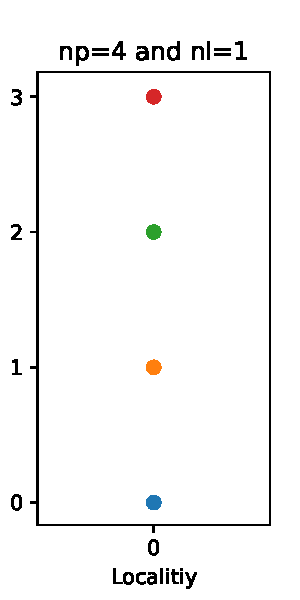
\includegraphics[width=\textwidth]{./images/partition2}
    \end{subfigure}
    ~ %add desired spacing between images, e. g. ~, \quad, \qquad, \hfill etc. 
      %(or a blank line to force the subfigure onto a new line)
    \begin{subfigure}[b]{0.3\textwidth}
        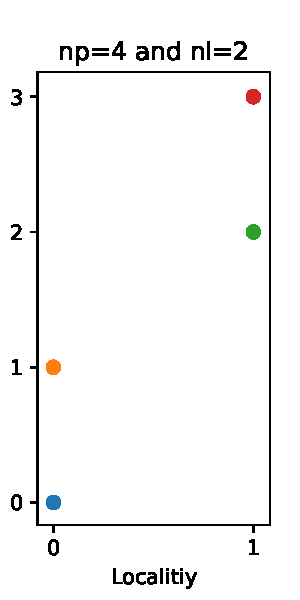
\includegraphics[width=\textwidth]{./images/partition1}
    \end{subfigure}
    ~ %add desired spacing between images, e. g. ~, \quad, \qquad, \hfill etc. 
    %(or a blank line to force the subfigure onto a new line)
    \begin{subfigure}[b]{0.3\textwidth}
        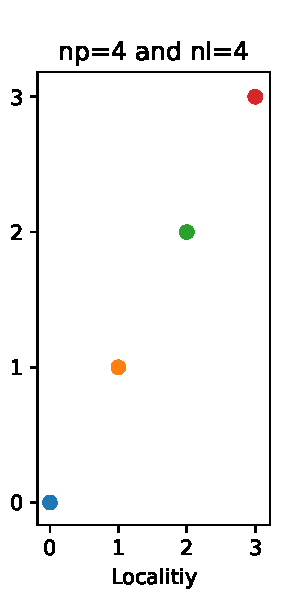
\includegraphics[width=\textwidth]{./images/partition3}
    \end{subfigure}
\end{figure}

\end{frame}

%%%%%%%%%%%%%%%%%%%%%%%%%%%%%%%%%%%%%%%%%%%%%%%%%%%%%%%%%%%%%%%%%%%%%%%%%%%%%%
\section{Scaling results}
%%%%%%%%%%%%%%%%%%%%%%%%%%%%%%%%%%%%%%%%%%%%%%%%%%%%%%%%%%%%%%%%%%%%%%%%%%%%%%

\begin{frame}[fragile]{Configuration file}

\begin{lstlisting}[language=bash]
#!/usr/bin/env bash

#SBATCH -o hostname_%j.out
#SBATCH -t 00:25:00
#SBATCH -p medusa
#SBATCH -D /home/pdiehl/Compile/hpx-1.3.0/build/bin/
export LD_LIBRARY_PATH
  =$LD_LIBRARY_PATH:
  /home/pdiehl/Compile/hpx-1.3.0/build/lib

module load gcc/8.2.0 boost/1.69.0-gcc8.2.0-release 
	mpi/openmpi-x86_64   

srun 1d_stencil_6 --nx=1000000 --np=10 
\end{lstlisting}

\begin{block}{Running}
\lstinline| sbatch -N 1,2,3,4,5 stencil.sbatch|
\end{block}

\end{frame}

\begin{frame}{Distributed scaling}

\begin{center}
\begin{tikzpicture}
\selectcolormodel{gray}
\begin{axis}[xlabel=Localities,ylabel=Execution time, grid=both,title=Stencil 6,legend style={at={(0.5,0.5)},anchor=west}]
\addplot table [x=Localities, y=Execution_Time_sec, col sep=comma] {./data/stencil_6.dat};
\end{axis}
\end{tikzpicture}
\end{center}
\end{frame}

%%%%%%%%%%%%%%%%%%%%%%%%%%%%%%%%%%%%%%%%%%%%%%%%%%%%%%%%%%%%%%%%%%%%%%%%%%%%%%
\section{Summary}
%%%%%%%%%%%%%%%%%%%%%%%%%%%%%%%%%%%%%%%%%%%%%%%%%%%%%%%%%%%%%%%%%%%%%%%%%%%%%%
\begin{frame}{Summary}
\begin{block}{After this lecture, you should know}
\begin{itemize}
\item How to compile HPX using networking
\item Receiving topology information
\end{itemize}
\end{block}
\end{frame}

%%%%%%%%%%%%%%%%%%%%%%%%%%%%%%%%%%%%%%%%%%%%%%%%%%%%%%%%%%%%%%%%%%%%%%%%%%%%%%
\section{References}
%%%%%%%%%%%%%%%%%%%%%%%%%%%%%%%%%%%%%%%%%%%%%%%%%%%%%%%%%%%%%%%%%%%%%%%%%%%%%%

\begin{frame}[t, allowframebreaks]
\frametitle{References}
\bibliographystyle{plain}
\bibliography{bib}
\end{frame}

\end{document}